\documentclass{article}
\usepackage{amsmath}
\usepackage{amssymb}
\usepackage{fancyhdr}
\usepackage[utf8]{inputenc}
\usepackage{tcolorbox}
\usepackage[left=1in, right=1in, top=1.5in, bottom=1in]{geometry}
\usepackage{tikz}
\usepackage{enumerate}
\usepackage{enumitem}

% Set up custom header
\pagestyle{fancy}
\tcbuselibrary{skins} % For advanced options like rounded corners
\fancyhf{} % Clear all header and footer fields
\fancyhead[L]{Your Name} % Left header with name
\fancyhead[R]{September 2nd 2025} % Right header with date
\renewcommand{\headrulewidth}{0.4pt} % Horizontal line below the header

\begin{document}

% Main title
\begin{center}
    \Large \textbf{Math 115E Activity 2} \\
    \vspace{0.2cm}
    \normalsize Chapter 2 Section 1 \\
    \normalsize The Coordinate System
\end{center}
\vspace{1cm} % Add space between the title and the first exercise

\textbf{Introduction to Intercepts of a graph and how to identify them}

\begin{tcolorbox}[
    width=\linewidth,
    colframe=black,         % Border color
    colback=white,          % Background color
    boxrule=0.5pt,          % Border thickness
    left=1mm, right=1mm,    % Horizontal padding
    top=1mm, bottom=1mm,    % Vertical padding
    arc=2mm                 % Corner radius
]
\textbf{Definition.} \textit{Given a graph in the coordinate plane, coordinate points of the form (x,0) on the curve are x-intercepts, and coordinate points of the form (0,y) on the curve are y-intercepts.}
\end{tcolorbox}

\noindent
\begin{minipage}[c]{0.45\textwidth}
    \begin{enumerate}
        
        \item For graph (A) what are the x-intercepts and y-intercepts?
        \vspace{2cm}
        \item For graph (B) what are the x-intercepts and y-intercepts?
        \vspace{2cm}
        \item For graph (C) what are the x-intercepts and y-intercepts?     
        \vspace{2cm}
        \item For graph (D) what are the x-intercepts and y-intercepts?
        

    \end{enumerate}
\end{minipage}%
\hfill
\begin{minipage}[c]{0.50\textwidth} % Minipage for the TikZ graph (increased width slightly for labels)
    \centering % Center the TikZ picture within its minipage
    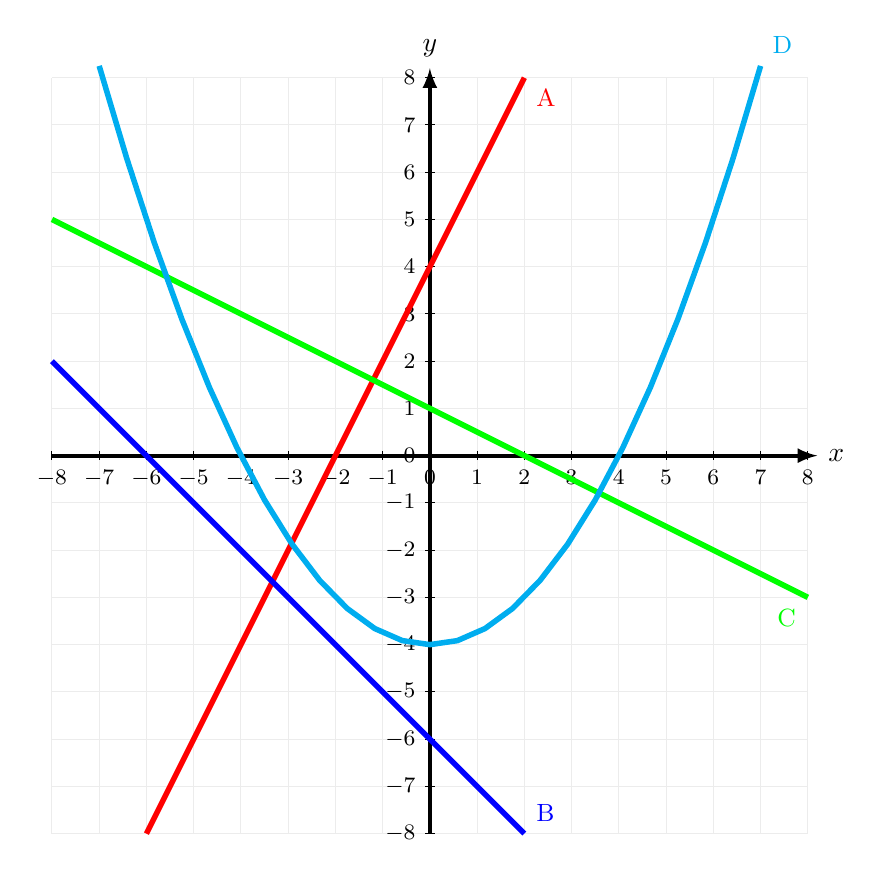
\begin{tikzpicture}[scale=0.60]
        \draw[gray!15,step=1cm] (-8,-8) grid (8,8);
        \draw[line width=0.5mm, -latex] (-8,0) -- (8.2,0) node[right] {$x$};
        \foreach \x in {-8,...,8} \draw (\x,.1)--(\x,-.1) node[below] {\footnotesize $\x$};
        \draw[line width=0.5mm,  -latex] (0,-8) -- (0,8.2) node[above] {$y$};
        \foreach \y in {-8,...,8} \draw (.1,\y)--(-.1,\y) node[left] {\footnotesize $\y$};

        % Red line with label 'a'
        \draw[red,line width=2pt] plot[domain= -6:2] (\x,{2*\x+4}) node[below right, font=\small] {A};
        % Blue line with label 'b'
        \draw[blue,line width=2pt] plot[domain= -8:2] (\x,{-1*\x-6}) node[above right, font=\small] {B};
        % Green line with label 'c'
        \draw[green,line width=2pt] plot[domain= -8:8] (\x,{-0.5*\x+1}) node[below left, font=\small] {C};
        % Cyan line with label 'd'
        \draw[cyan,line width=2pt] plot[domain= -7:7] (\x,{0.25*\x*\x-4}) node[above right, font=\small] {D};
    \end{tikzpicture}
\end{minipage}

\vspace{10cm}
\begin{center}
    \Large \textbf{Math 115E Activity 2} \\
    \vspace{0.2cm}
    \normalsize Chapter 2 Section 2 \\
    \normalsize What are Functions?

\end{center}

\vspace{1cm}
\textbf{How to interpret intercepts from a function table} \\
\begin{enumerate}[label=\textbf{\arabic*.}]
\item A balloon is rising from a ravine, it starts 13 ft below ground (fill in the missing values)
\begin{center}
\begin{tabular}{ |c|c|c|c|c|c|c|c|c|c|c|c| } 
 \hline
 $t \; (sec)$ & 0 & 2 & 4 & \hspace{0.35cm} & 8 & \hspace{0.35cm} & 12 & 14 & \hspace{0.35cm} & 18 & 20 \\
 \hline
 $f(t) \; (feet)$ & -13 & \hspace{0.35cm} & -9 & -7 & -5 & -3 & \hspace{0.35cm} & 1 & 3 & \hspace{0.35cm} & 7\\ 
 \hline

\end{tabular}
\end{center}
\begin{enumerate}[label=\textbf{\alph*.}]
    \item What is the value of $f(12)$ and $f(2)$. What does it represent?
    \vspace{1.25cm}
    \item What is the hight of the balloon at $time=4$
    \vspace{1.25cm}
    \item What time does the balloon reach ground level?    
    \vspace{1.25cm}
    \item When does the balloon reach $10$ feet below ground?

\end{enumerate}
\vspace{1cm}
\item A ball is falling from the sky, then bounces off the ground then falls back down and stops
\begin{center}
\begin{tabular}{ |c|c|c|c|c|c|c|c|c|c|c|c| } 
 \hline
 $t \; (sec)$ & 0 & 1 & 2 & 3 & 4 & 5 & 6 & 7 & 8 & 9 & 10 \\
 \hline
 $g(t) \; (feet)$ & 12 & 9 & 6 & 3 & 0 & 3 & 6 & 9 & 6 & 3 & 0\\ 
 \hline

\end{tabular}
\end{center}
\begin{enumerate}[label=\textbf{\alph*.}]
    \item What is the value of $f(4)$ and $f(9)$ what does it represent?
    \vspace{1.25cm}
    \item What is the height of the balloon at $time=6$
    \vspace{1.25cm}
    \item How many times does the ball touch the ground?  
    \vspace{1.25cm}
    \item What are the x-intercepts and y-intercepts?
\end{enumerate}
\end{enumerate}
\end{document}